\documentclass[conference]{IEEEtran}
\usepackage{amsmath,graphicx,booktabs,tabularx,array,cite,booktabs,subcaption}
\usepackage[normalem]{ulem}
\usepackage{hyperref}
\newcolumntype{Y}{>{\centering\arraybackslash}X}

\title{Deep Learning for Satellite Image Semantic Segmentation}
\author{
    \IEEEauthorblockN{Chinatip Lawansuk}
    \IEEEauthorblockA{
        Department of Electrical Engineering and Computer Science\\
        National Taipei University of Technology\\
        Email: t112998405@ntut.edu.tw
    }
}

\begin{document}

\maketitle

\begin{abstract}
Aerial image semantic segmentation is a crucial task in remote sensing and geographic information systems (GIS). This report provides an overview of methods and techniques used in semantic segmentation of aerial images, discusses the challenges involved, and highlights recent advancements in the field. Utilising the U-Net architecture and its deep variants, we demonstrate how these models address limitations of traditional methods by improving accuracy and efficiency in land use surveys. Our study includes a performance comparison of different activation functions, with ReLu achieving the highest Mean IoU at 0.896, followed by Leaky ReLu at 0.829, and Tanh at 0.763. We also compare Multiple Model Single Channel (MMSC) and Single Model Multiple Channel (SMMC) architectures, finding SMMC more effective with 8.45 million parameters and 32.27 MB memory usage. Real-world application on Google Maps data showcases the model’s capabilities and areas for improvement, emphasising its potential for urban planning, environmental monitoring, and resource management.
\end{abstract}

\section{Introduction}
Surveying land usage is critical for sustainable development, environmental conservation, and efficient resource management. Traditional land surveying techniques, while foundational, are often limited by their scalability, accuracy, and reliance on extensive human intervention. The advent of aerial imagery has revolutionised this field, offering high-resolution and comprehensive coverage of vast areas, significantly enhancing the efficiency and accuracy of land surveys. However, interpreting these images using traditional algorithms, such as manual interpretation, supervised and unsupervised classification, edge detection, and segmentation, poses challenges including high labour costs, human error, and sensitivity to data variability.

In recent years, deep learning, particularly convolutional neural networks (CNNs), has emerged as a powerful tool for image segmentation. Among these, the U-Net architecture stands out for its ability to combine high-level contextual information with precise localisation, making it particularly effective for complex image segmentation tasks. U-Net's symmetric encoder-decoder structure, augmented with skip connections, facilitates the retention of fine-grained details, which is crucial for accurately delineating land features in aerial imagery. Enhanced variants such as Deep U-Net further improve segmentation accuracy by incorporating deeper networks and advanced techniques like attention mechanisms and multi-scale processing.

This work explores the application of U-Net and its deep variants in the segmentation of aerial images, demonstrating how these architectures address the limitations of traditional methods. Additionally, we focus on the critical aspects of data preparation and preprocessing, which are essential for improving the performance of deep learning models. Proper data preparation, including tasks such as noise reduction, image enhancement, and augmentation, ensures that the models are trained on high-quality datasets, thereby enhancing their robustness and generalisation capabilities.

By leveraging the strengths of deep learning and thorough data preparation, this approach aims to enhance the precision, scalability, and efficiency of land use surveys, ultimately contributing to better-informed decision-making in urban planning, environmental monitoring, and resource management.

\section{Dataset}
In our work, we utilise the dataset titled "Semantic Segmentation of Aerial Imagery", which comprises 72 high-resolution aerial images. Each image in this dataset is up to 1800$\times$2000 pixels, providing a substantial amount of detail for our analysis. The dataset can be accessed via the following link: \href{https://www.kaggle.com/datasets/humansintheloop/semantic-segmentation-of-aerial-imagery}{https://www.kaggle.com/datasets/humansintheloop/semantic-segmentation-of-aerial-imagery}.

\begin{figure*}[!h]
    \centering
    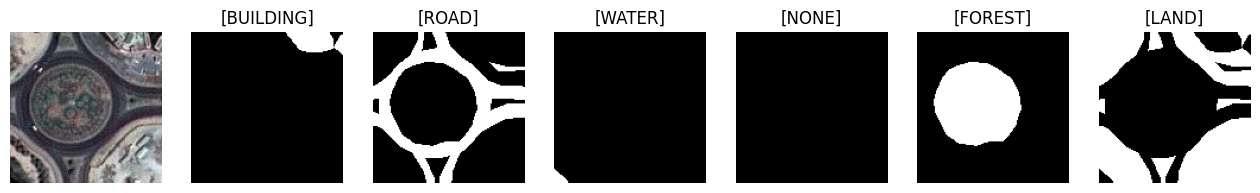
\includegraphics[width=\textwidth]{data_prep.png}
    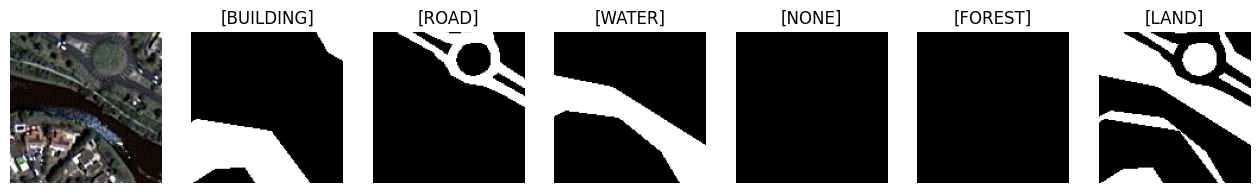
\includegraphics[width=\textwidth]{data_prep2.png}
    \caption{Dataset shows original image and splitted masks}
    \label{fig:data_set}
\end{figure*}

\subsection*{Data Preprocessing}
\subsubsection{Crop}
To enhance training efficiency, we randomly select a point on the image and crop a 128$\times$128 patch, using the selected point as the top-left corner of the cropped image. This method ensures diverse and representative samples, capturing various features and contexts from the original images. As shown in Fig. \ref{fig:data_set}.

\subsubsection{Split}
For the split, the original RGB mask, with different colours for each type, is split into 6 binarised black-white images, each representing a specific class. These binary images are combined to form a 6 channels input when loading into the model, allowing it to process each class separately and effectively. As shown in Fig. \ref{fig:data_set}

Additionally, we have published the processed dataset on Kaggle for sharing, allowing others to cite it in their work. The dataset can be accessed at \href{https://www.kaggle.com/datasets/lchinatip/aerial-image-dataset-for-semantic-segmentation/data}{https://www.kaggle.com/datasets/lchinatip/aerial-image-dataset-for-semantic-segmentation/data}.

\section{Model Architecture}

In this work, we utilise the U-Net model, delving into both its architectural design and activation functions. By optimising these aspects, we aim to enhance the model's performance and accuracy in image segmentation tasks. Our exploration includes experimenting with various configurations to identify the most effective combination for our specific applications.

\subsection{Specifications and Constraints}
\begin{itemize}
    \item Input Layer Dimension: 128$\times$128 pixels
    \item Input Layer Channel: 3 channels (RGB)
    \item Convolution Depth: 4 (Feature Maps from 64, 128, 256, 512)
    \item Output Layer Dimension: 128$\times$128 pixels
    \item Output Layer Channel: 6 channels (Multiclass)
    \item Model Optimisation: Adam
    \item Training Epoch : 5000
\end{itemize}
\subsection{Architectural Design}
\subsubsection{Multiple Model Single Channel (MMSC)}
This approach involves using multiple submodels, each dedicated to a single class. As shown in Fig. \ref{fig:multiple}.

\subsubsection{Single Model Multiple Channel (SMMC)}
In this approach, a single model is designed to have multiple channels on each layer, representing a different class. As shown in Fig. \ref{fig:single}.

We then evaluate the model, as shown in Table \ref{tab:model_compare_dims}.

\begin{figure*}[t!]
    \centering
    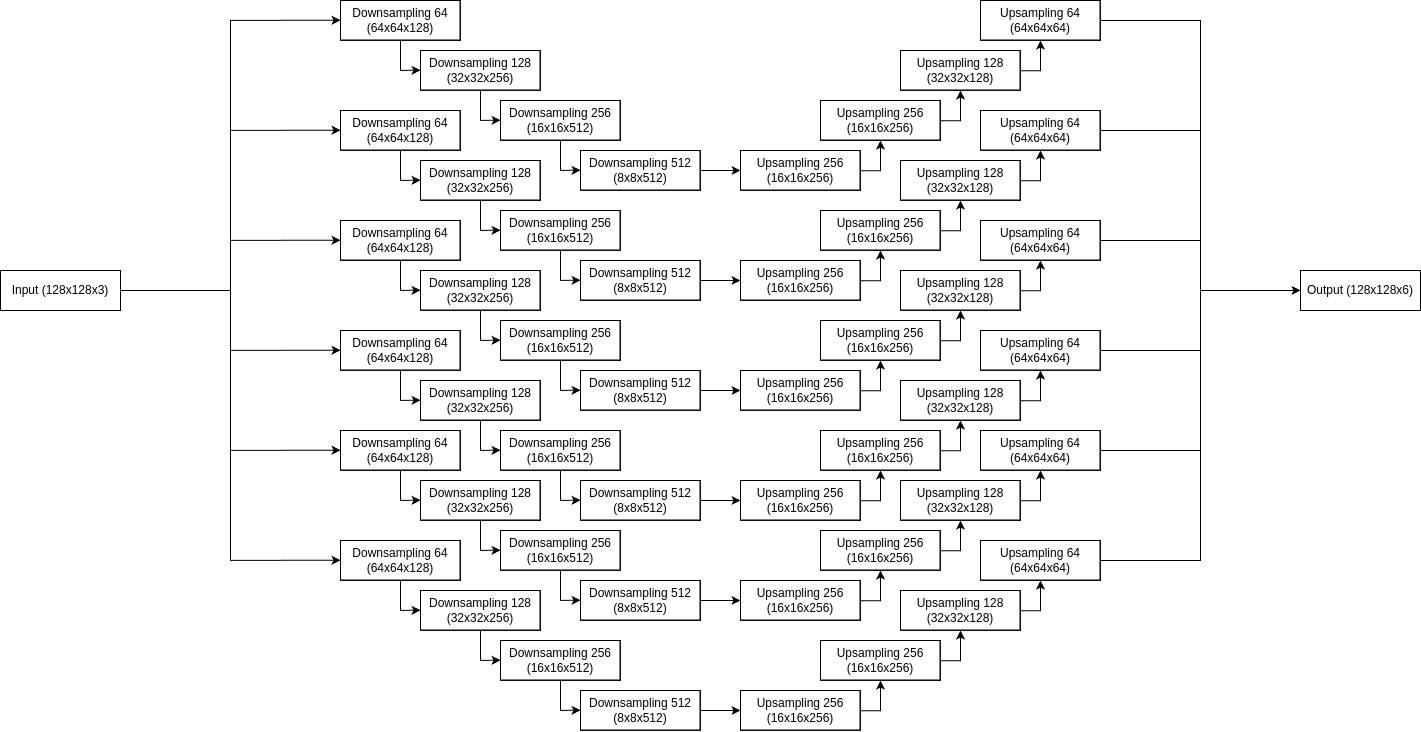
\includegraphics[width=\textwidth]{multiple_model.png} % Replace with your image file
    \caption{Multiple Model Single Channel (MMSC)}
    \label{fig:multiple}
\end{figure*}

\begin{figure}[t!]
    \centering
    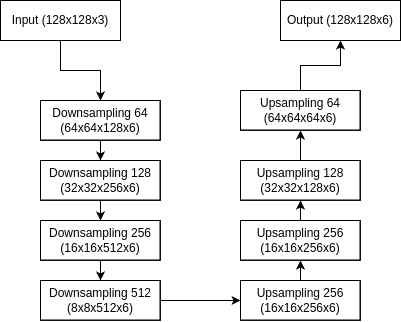
\includegraphics[width=\columnwidth]{single_model.png} % Replace with your image file
    \caption{Single Model Multiple Channel (SMMC)}
    \label{fig:single}
\end{figure}

\begin{table}[h!]
    \centering
    \caption{Model Comparison Between Multiple Model Single Channel (MMSC) and Single Model Multiple Channel (SMMC)}
    \label{tab:model_compare_dims}
    
    \begin{tabularx}{\columnwidth}{|c|Y|Y|}
        \hline
        \textbf{Properties} & \textbf{MMSC} & \textbf{SMMC} \\
        \hline
        Parameters & 12.47 M & 8.45 M \\
        \hline
        Memory & 47.59 MB & 32.27 MB \\
        \hline
    \end{tabularx}
\end{table}

The Multiple Model Single Channel approach takes smaller parameter count and memory usage compared to the Single Model Multiple Channel method. This is because the former splits the task into 6 distinct submodules, each handling a single channel, resulting in smaller individual models. However, training the Multiple Model Single Channel configuration takes more time since it requires updating gradients 6 times, once for each submodule.

In contrast, the Single Model Multiple Channel approach, despite being larger, tends to yield better performance. This improvement is primarily due to fully connected among each channel, as it maintains the interconnection between different classes within a unified model. The Multiple Model Single Channel setup lose these interconnections, which can lead to suboptimal performance. By preserving the relationships between classes, the Single Model Multiple Channel approach can achieve more accurate and coherent segmentation results. Resulting in lower overlaps output among the channel.

Hence, We decided to use the Single Model Multiple Channel.
\subsection{Activation Functions}

As shown in the model architecture in Fig . Each layer is consisted of Activation layer. We work on multiple activation functions to evaluate the characteristic and performance.

\subsubsection{ReLu}
Rectified Linear Unit is a popular yet simple activation function in neural networks. ReLu introduces non-linearity into the model, enabling the learning of complex patterns. It is computational efficiency, due to the simple operations, and it is able to mitigate the vanishing gradient problem.
\[
\text{ReLu}(x) = \max(0, x)
\]

\subsubsection{Leaky ReLu}
Leaky ReLu is is a variant of the ReLu activation function. It allows a small, non-zero gradient when the input is negative. This addresses the dying ReLu problem by ensuring that neurons do not become inactive. Leaky ReLu introduces slight non-linearity, improving model performance and convergence.

\[
\text{LeakyReLu}(x) = 
\begin{cases} 
x & \text{if } x \geq 0 \\
\alpha x & \text{if } x < 0 
\end{cases}
\]

\subsubsection{Tanh}
Tanh It maps input values to a range between -1 and 1, providing zero-centered outputs. Tanh introduces non-linearity, enabling the model to capture complex patterns. It also helps mitigate the vanishing gradient problem compared to the sigmoid function.

\[
\text{tanh}(x) = \frac{e^x - e^{-x}}{e^x + e^{-x}}
\]

\section{Metrics and Evaluation}
We introduce the metrics of our model and evaluation method that had been use in our work.

\subsection{Pixel-wise Accuracy}

Pixel-wise accuracy is a metric used to evaluate the performance of image segmentation models. It measures the proportion of correctly classified pixels over the total number of pixels in an image or set of images. Mathematically, it is defined as
\[
\text{Pixel-wise Accuracy} = \frac{\text{No. Correctly Classified Pixels}}{\text{Total No. of Pixels}}
\]
This metric provides a straightforward way to assess how well the segmentation model distinguishes between different regions or objects within an image. High pixel-wise accuracy indicates that the model effectively assigns the correct labels to most pixels, leading to precise and reliable segmentation results.

\subsection{Mean Intersect over Union (MeanIoU)}

Mean Intersection over Union (Mean IoU) is a performance metric for image segmentation models. It measures the average overlap between predicted and ground truth segments across all classes. IoU is calculated as the intersection of predicted and true regions divided by their union. Mean IoU, the average IoU across all classes, provides a robust evaluation by accounting for both false positives and false negatives, reflecting model accuracy comprehensively.

\[
\text{Mean IoU} = \frac{1}{N} \sum_{i=1}^{N} \frac{|A_i \cap B_i|}{|A_i \cup B_i|}
\]

\text{where:} \\
$N$ \text{ is the number of classes} \\
$A_i$ \text{ is the set of pixels in the predicted mask for class } i \\
$B_i$ \text{ is the set of pixels in the ground truth mask for class } i

for intersection,

\[
A \cap B = \sum_{i} a_i \wedge  b_i
\]
and union,
\[
A \cup B = \sum_{i} a_i \vee  b_i
\]

\[
\text{IoU} = \frac{\sum_{i} a_i \cdot b_i}{\sum_{i} (a_i + b_i - a_i \cdot b_i)}
\]


\text{where:} \\
$a_i$ \text{ is binarised value of the i-th pixel in the predicted mask} \\
$b_i$ \text{ is binarised value of the i-th pixel in the ground truth mask}




\subsection{RMSE}
Root Mean Square Error (RMSE) is a widely used metric for evaluating the accuracy of a model's predictions. It measures the square root of the average of the squared differences between the predicted and actual values. RMSE provides a way to quantify the difference between predicted and observed values, with lower values indicating better model performance. It is particularly useful because it gives a high penalty to large errors, making it sensitive to outliers.

\[
\text{RMSE} = \sqrt{\frac{1}{n} \sum_{i=1}^{n} (a_i - \hat{b}_i)^2}
\]

\text{where:} \\
$a_i$ \text{ is the actual values} \\
$b_i$ \text{ is the predicted values} \\
$n$ \text{ is the number of pixel}

\subsection*{Loss function}
We customise Loss function to serve our own work. This is done by combine MeanIoU with RMSE with different ratio.

\subsection*{Metric}
We prefer using Validation MeanIoU to be a key for tracking the performance. Since it gives overview performance of a model among all channel.


\section{Results}
\subsection{Performance Comparison}

\begin{table}[h!]
    \centering
    \caption{Model Comparison Between Multiple Model Single Channel (MMSC) and Single Model Multiple Channel (SMMC)}
    \label{tab:model_compare_perf}
    
    \begin{tabularx}{\columnwidth}{|Y|Y|}
        \hline
        \textbf{Model} & \textbf{MeanIoU} \\
        \hline
        ReLu & 0.896  \\
        \hline
        LeakyReLu & 0.829  \\
        \hline
        tanh & 0.763  \\
        \hline
    \end{tabularx}
\end{table}

\begin{figure*}[h!]
    \centering
    \begin{subfigure}[b]{\textwidth}
        \centering
        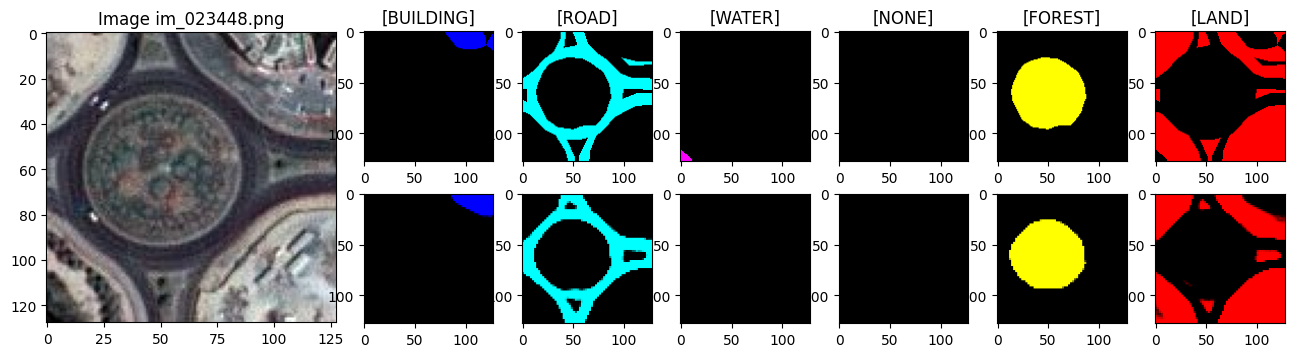
\includegraphics[width=\textwidth]{relu_5000.png} 
        \caption{Prediction Result From ReLu model}
        \label{fig:res_relu}
    \end{subfigure}
    \begin{subfigure}[b]{\textwidth}
        \centering
        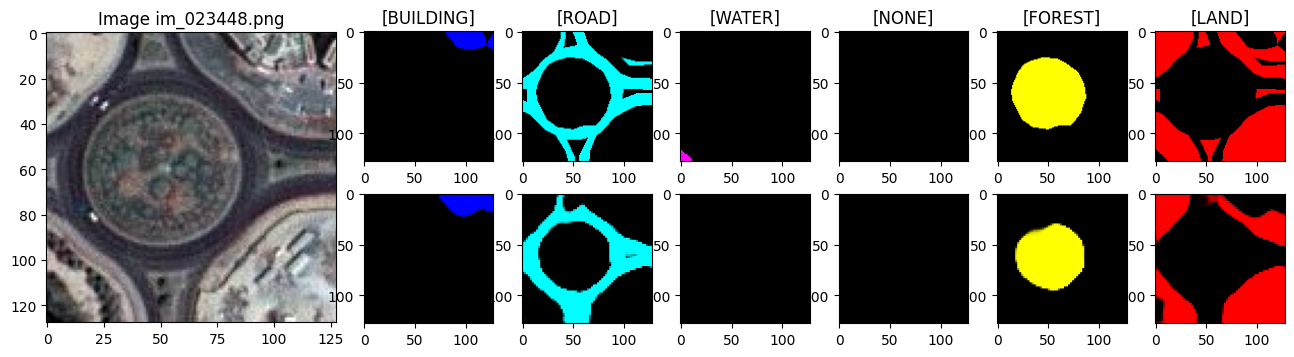
\includegraphics[width=\textwidth]{leaky_5000.png} 
        \caption{Prediction Result From LeakyReLu model}
        \label{fig:res_leaky}
    \end{subfigure}
    \begin{subfigure}[b]{\textwidth}
        \centering
        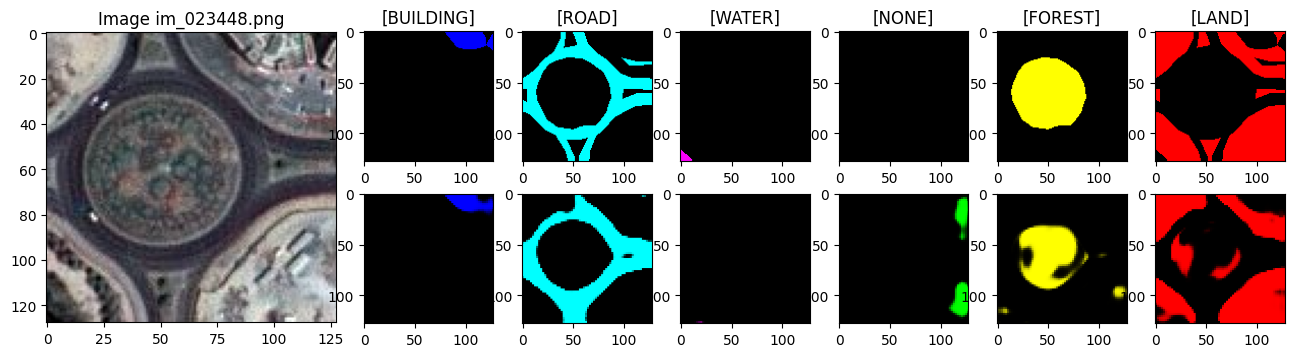
\includegraphics[width=\textwidth]{tanh_5000.png} % Replace with your image file
        \caption{Prediction Result From tanh model}
        \label{fig:res_tanh}
    \end{subfigure}
    \caption{Prediction result from various model}
    \label{fig:multiple}
\end{figure*}

In this evaluation of mean Intersection over Union (Mean IoU), the Rectified Linear Unit (ReLu) activation function delivered the best performance with a Mean IoU of 0.896. This high score reflects ReLu's ability to facilitate robust and stable learning, contributing to accurate segmentation results. As shown in Fig. \ref{fig:res_relu}. In contrast, the Leaky Rectified Linear Unit (Leaky ReLu) showed slightly lower performance, achieving a Mean IoU of 0.829. As shown in Fig. \ref{fig:res_leaky}. Although Leaky ReLu addresses the "dying ReLu" problem, it still falls short of ReLu's superior performance. The hyperbolic tangent (tanh) activation function performed the worst among the three, with a Mean IoU of 0.763. As shown in Fig. \ref{fig:res_tanh}. This lower score highlights tanh's inconsistency and slower convergence, making it less effective for precise segmentation tasks. As shown in Table \ref{tab:model_compare_perf}.

\subsection{Performance on Training}
In this work, we observed that the Rectified Linear Unit (ReLu) activation function delivered the best performance among the tested activation functions. ReLu not only facilitated faster convergence but also maintained stability throughout the training epochs. This consistency is likely due to ReLu’s inherent ability to mitigate the vanishing gradient problem, ensuring that the model learns effectively even in deep networks. As shown in \ref{fig:perf_relu}.
\begin{figure}[h]
    \centering
    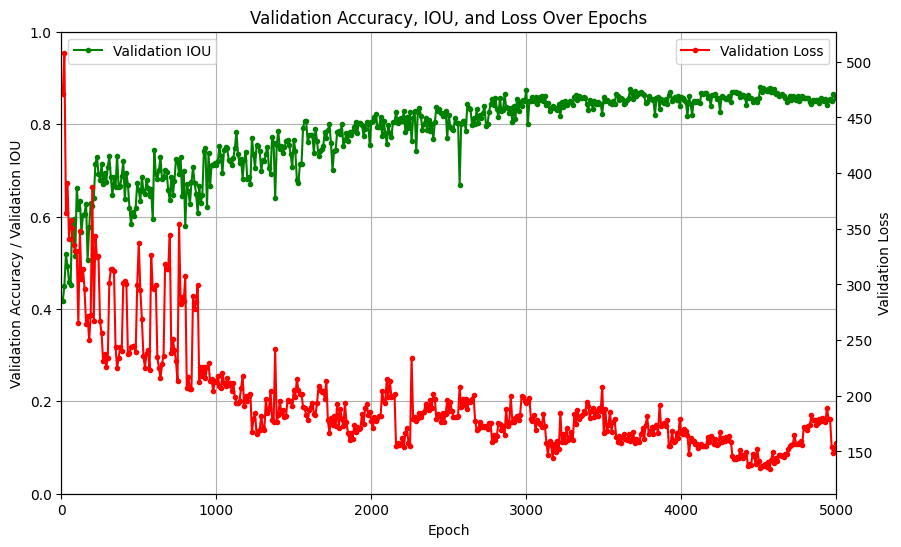
\includegraphics[width=\columnwidth]{relu_perf.png} % Replace with your image file
    \caption{MeanIoU over Training Epoch for ReLu}
    \label{fig:perf_relu}
\end{figure}
On the other hand, the Leaky Rectified Linear Unit (Leaky ReLu) showed a slightly slower convergence compared to ReLu. Although it addressed the "dying ReLu" problem by allowing a small, non-zero gradient when the input is negative, this modification did not translate into faster learning. Despite this, Leaky ReLu performed reasonably well and maintained a relatively stable mean Intersection over Union (Mean IoU) metric, although not as consistently as ReLu. As shown in \ref{fig:perf_leaky}.
\begin{figure}[!t]
    \centering
    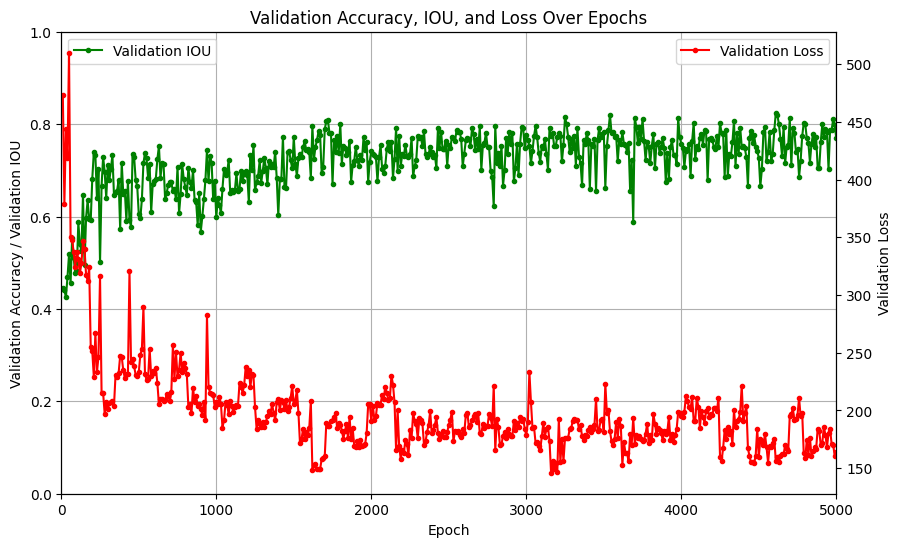
\includegraphics[width=\columnwidth]{leaky_perf.png} % Replace with your image file
    \caption{MeanIoU over Training Epoch for LeakyReLu}
    \label{fig:perf_leaky}
\end{figure}
Conversely, the tanh activation function gave the poorest performance in our tests. Tanh not only converged the slowest but also showed significant inconsistency throughout the training process. The Mean IoU for tanh fluctuated dramatically, alternately rising and dropping sharply across epochs. This volatility suggests that tanh struggles to maintain a stable learning trajectory, possibly due to its outputs saturating at large values, which worsen the vanishing gradient problem. As shown in \ref{fig:perf_tanh}.
\begin{figure}[!t]
    \centering
    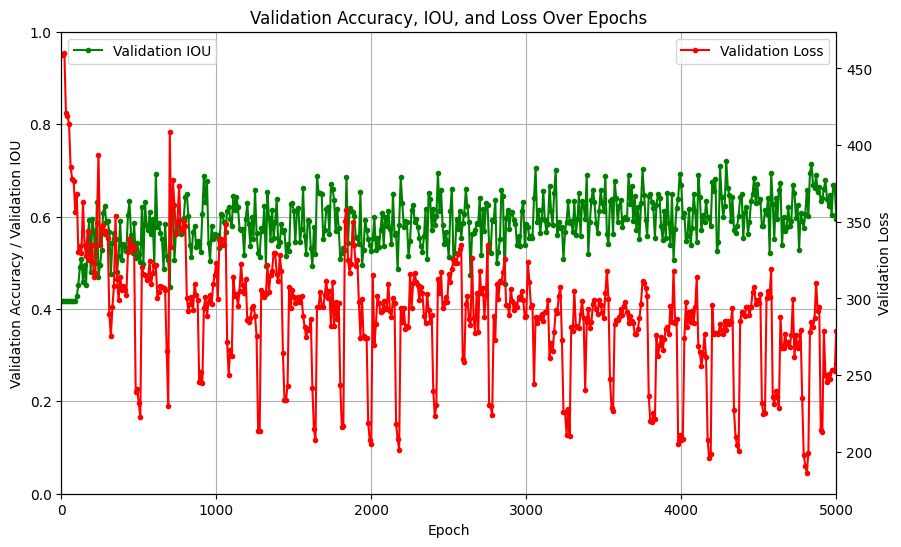
\includegraphics[width=\columnwidth]{tanh_perf.png} % Replace with your image file
    \caption{MeanIoU over Training Epoch for tanh}
    \label{fig:perf_tanh}
\end{figure}

Both Leaky ReLu and tanh demonstrated inconsistency in their Mean IoU metrics during the training epochs. Unlike ReLu, whose performance was consistently robust, Leaky ReLu and tanh alternately rose and fell in their Mean IoU, indicating unstable learning dynamics. This instability can hinder the overall effectiveness of the model, making these activation functions less desirable.





\section{Application}
\subsection{Application with Real Data from Google Maps}

In this work, we employed the ReLu model with real images sourced from Google Maps, using the Google Maps API. We tested the model on three locations: Shezi District, Abu Dhabi, and another diverse location. Shezi District, with its urban landscape surrounded by small forest areas and a river, presented a varied environment. Abu Dhabi's arid land adjacent to a river provided a stark contrast. The results indicated that the model effectively segmented major areas such as roads, water bodies, and vegetation. However, it struggled with high-detail classes like buildings, leading to segmentation errors. This discrepancy is likely due to the differing characteristics of buildings in Abu Dhabi and Shezi District, highlighting the model's limited tolerance to highly varied data. These findings suggest that while the model performs well overall, improvements are needed to enhance its accuracy for detailed structures across diverse landscapes.

\begin{figure*}[!h]
    \centering
    \begin{subfigure}[h]{\textwidth}
        \centering
        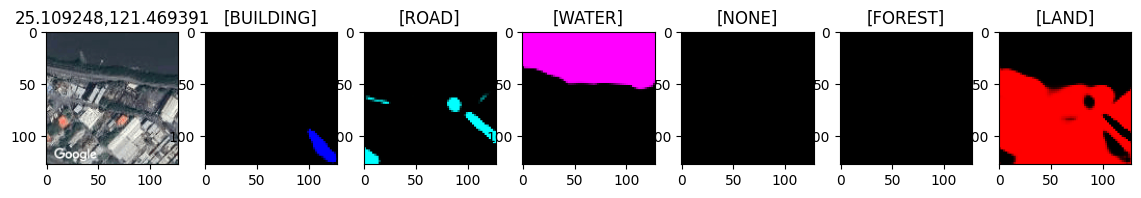
\includegraphics[width=\textwidth]{gmaps.png} 
        \caption{Prediction Result From Shezi area}
        \label{fig:shezi}
    \end{subfigure}
    \begin{subfigure}[h]{\textwidth}
        \centering
        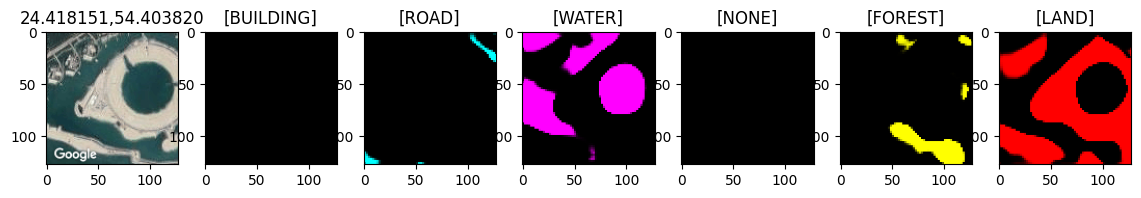
\includegraphics[width=\textwidth]{gmaps2.png} 
        \caption{Prediction Result for Abu Dhabi}
        \label{fig:abu_dhabi}
    \end{subfigure}
    \caption{Prediction result on real data from Google Maps}
    \label{fig:real_data}
\end{figure*}

\section{Conclusion}
We explore the application of deep learning techniques, particularly the U-Net architecture, for the semantic segmentation of aerial images. The study demonstrates the advantages of deep learning over traditional methods in terms of accuracy and efficiency. We compare the performance of different activation functions, with ReLu achieving the highest Mean IoU at 0.896, followed by Leaky ReLu at 0.829, and Tanh at 0.763. Through detailed data preparation and preprocessing, we ensure robust model training. The application of the model on real-world data from Google Maps showcases its potential in diverse environments, though it highlights the need for further improvements in segmenting highly detailed structures.

\bibliographystyle{IEEEtran}
\bibliography{references}

\end{document}
